\documentclass[10pt]{article}

\usepackage{spheric}
%%%TITLE
\title{A Physics Evoked Meshfree Method}
\date{}

%%AFFILIATIONS
\author[1]{MA Zhi-bo}
\author[2]{ZHAO Ya-zhou$^\dagger$}

\affil[1]{Institute of Applied Physics and Computational Mathematics, Beijing 100094, China}
\affil[2]{Institute of Geology and Geophysics, Chinese Academy of Science, Beijing 100029, China}

\affil[$\relax$]{\email{\dagger}{asiabuaasa@163.com}}


%%DOCUMENT
\begin{document}

\maketitle

%\SelectedTopics{}

%%PLEASE PUT YOUR ABSTRACT HERE
\begin{abstract}
In mesh free methods, discrete equations are built according to physics information of micro-bodies arbitrarily spread in vicinal space. As the requirements about topology of micro-bodies are reduced, simulations with Lagrangian approach may be easier even with large distortions. Owing to the insufficiency of topological information, there is a challenge for mesh-free method to reflect physics especially as discontinuities exist. Based on the physical laws and developing trend of numerical simulation, a new mesh free systematic method PECM (Physics Evoked Cloud Method) which has excellent applicability is shown. High fidelity to physics of the method is demonstrated through five 1-dimentional challenging problems in which strong discontinuities exist. 




\begin{figure}[!htb]
\centering
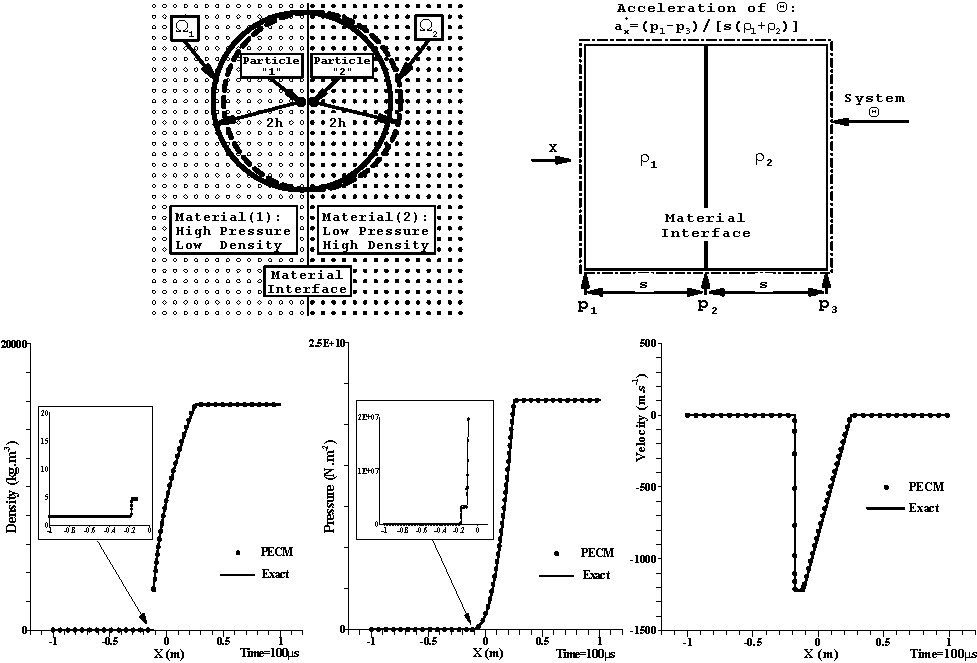
\includegraphics[width=0.95\textwidth]{56-1.pdf}
\caption{Kernel Modification in PECM (top) \& Validation of PECM(down): Numerical results about Case 5}\label{fig:}
\end{figure}

\end{abstract}


%%THE END OF ABSTRACT

\addbib

\end{document}
